% Copyright (c) 2010 Jérémie DECOCK (http://www.jdhp.org)

\documentclass[pdftex,a4paper,11pt]{article} 
%\documentclass[pdftex,a4paper,11pt]{report} 
\usepackage[utf8]{inputenc}
\usepackage[frenchb]{babel}
\usepackage[pdftex]{graphicx}
\usepackage{amsmath}
\usepackage{amssymb}
\usepackage{subfigure}
\usepackage{hyperref}

\hypersetup{
	pdftoolbar=true,                    % show Acrobat’s toolbar ?
	pdfmenubar=true,                    % show Acrobat’s menu ?
	pdffitwindow=true,                  % page fit to window when opened
	pdftitle={Pyarm},                   % title
	pdfauthor={Jérémie DECOCK},         % author
	pdfsubject={Pyarm},                 % subject of the document
	pdfnewwindow=true,                  % links in new window
	pdfkeywords={Pyarm},                % list of keywords
	colorlinks=true,                    % false: boxed links; true: colored links
	linkcolor=black,                    % color of internal links
	citecolor=black,                    % color of links to bibliography
	filecolor=black,                    % color of file links
	urlcolor=black                      % color of external links
}

%\newcommand{\reels}{\mathbb{R}}
\numberwithin{equation}{subsection}

\begin{document}

\title{Pyarm}
\author{
	Jérémie \bsc{Decock}
}
\date{\today{}}

\maketitle

%%%%%%%%%%%%%%%%%%%%%%%%%%%%%%%%%%%%%%%%%%%%%%%%%%%%%%%%%%%%%%%%%%%%%%%%%%%%%%%%

\section{Présentation des modèles}

\subsection{Présentation}

\begin{center}
        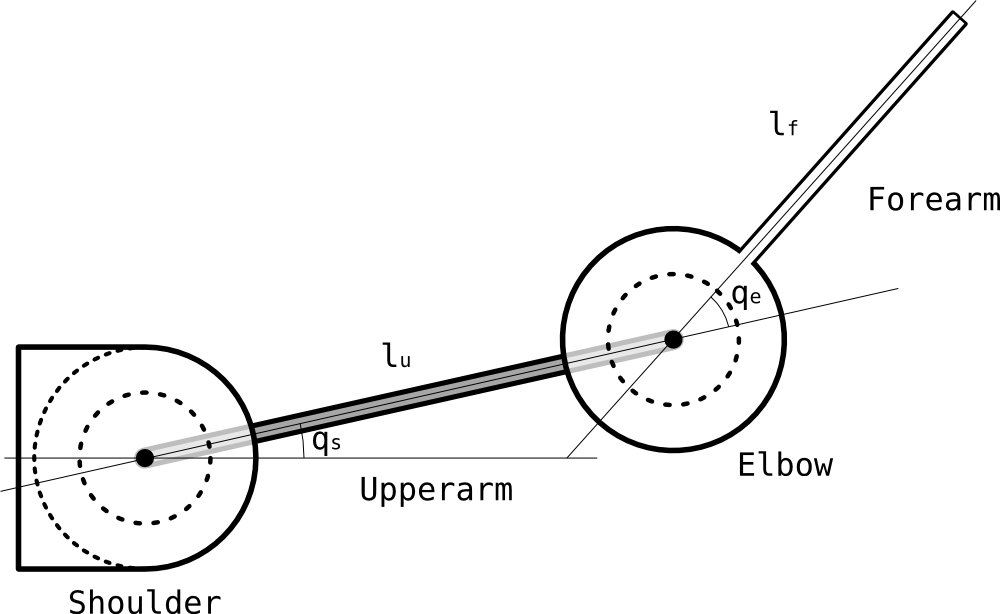
\includegraphics[width=.40\linewidth]{fig/arm}
\end{center}

\begin{itemize}
    \item Bras 2D
    \item Plan transverse (Mitrovic, Weiwei) ou sagittal (Kambara)
    \item 2 membres (le bras et l'avant-bras) % ou arrière-bras ou bras supérieur
    \item 2 articulations (épaule et coude)
    \item 6 muscles~:
    \begin{enumerate}
        \item fléchisseur de l'épaule
        \item extenseur de l'épaule
        \item fléchisseur du coude
        \item extenseur du coude
        \item double fléchisseur
        \item double extenseur
    \end{enumerate}
\end{itemize}

Remarque : la numérotation des muscles est différente dans le modèle de Weiwei.

\subsection{Les modèles étudiés}
Trois modèles ont été étudiés~:
\begin{itemize}
    \item Katayama / Mitrovic \cite{katayama1993, ozkaya1999, mitrovic10, mitrovic2008, mitrovic2009}
    \item Kambara \cite{kambara2009, ozkaya1999}
    \item Brown / Weiwei \cite{brown1999, li2006, li2004, todorov2005}
\end{itemize}

\subsection{Historique}

\begin{center}
        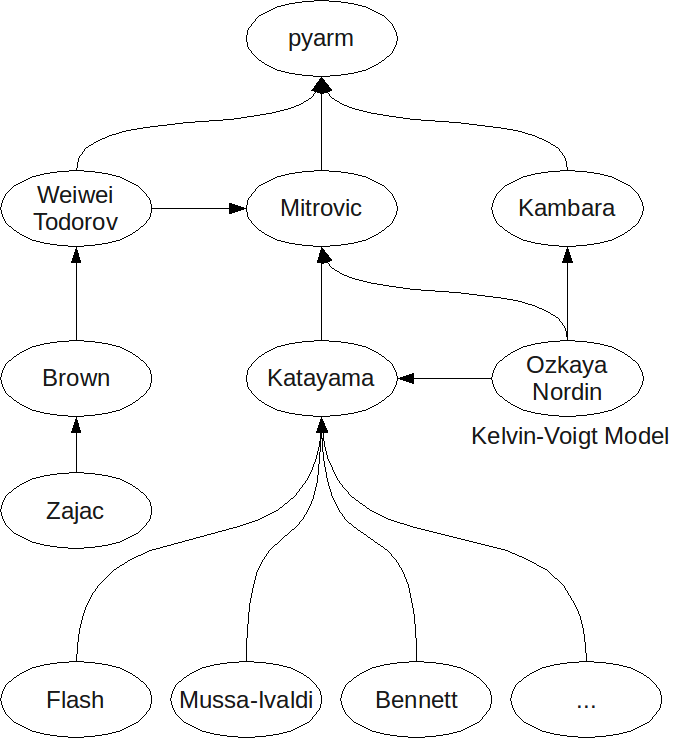
\includegraphics[width=.80\linewidth]{fig/bib}
\end{center}

\subsection{Simulateur Pyarm}

\begin{itemize}
    \item Codé en Python
    \item Implémente les 3 modèles
\end{itemize}

%\begin{center}
%    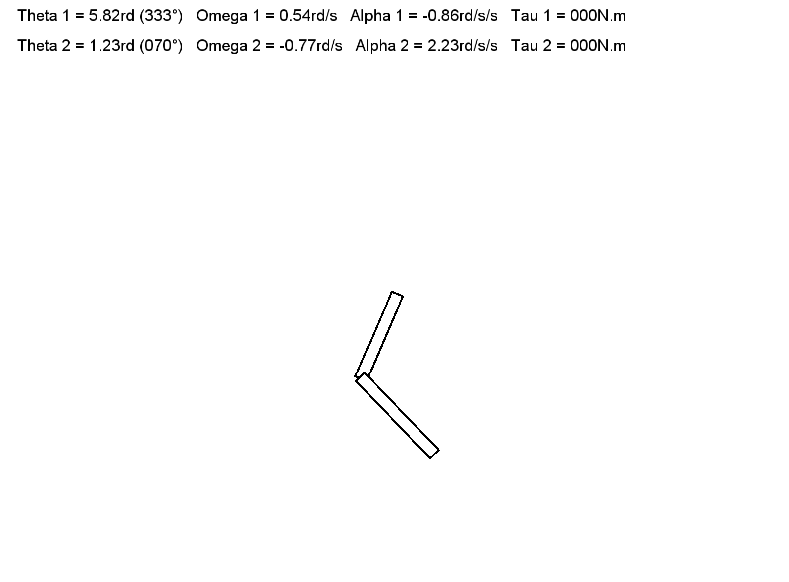
\includegraphics[width=.40\linewidth]{fig/pyarm1}
%\end{center}
\begin{figure}
    \centering
    \subfigure{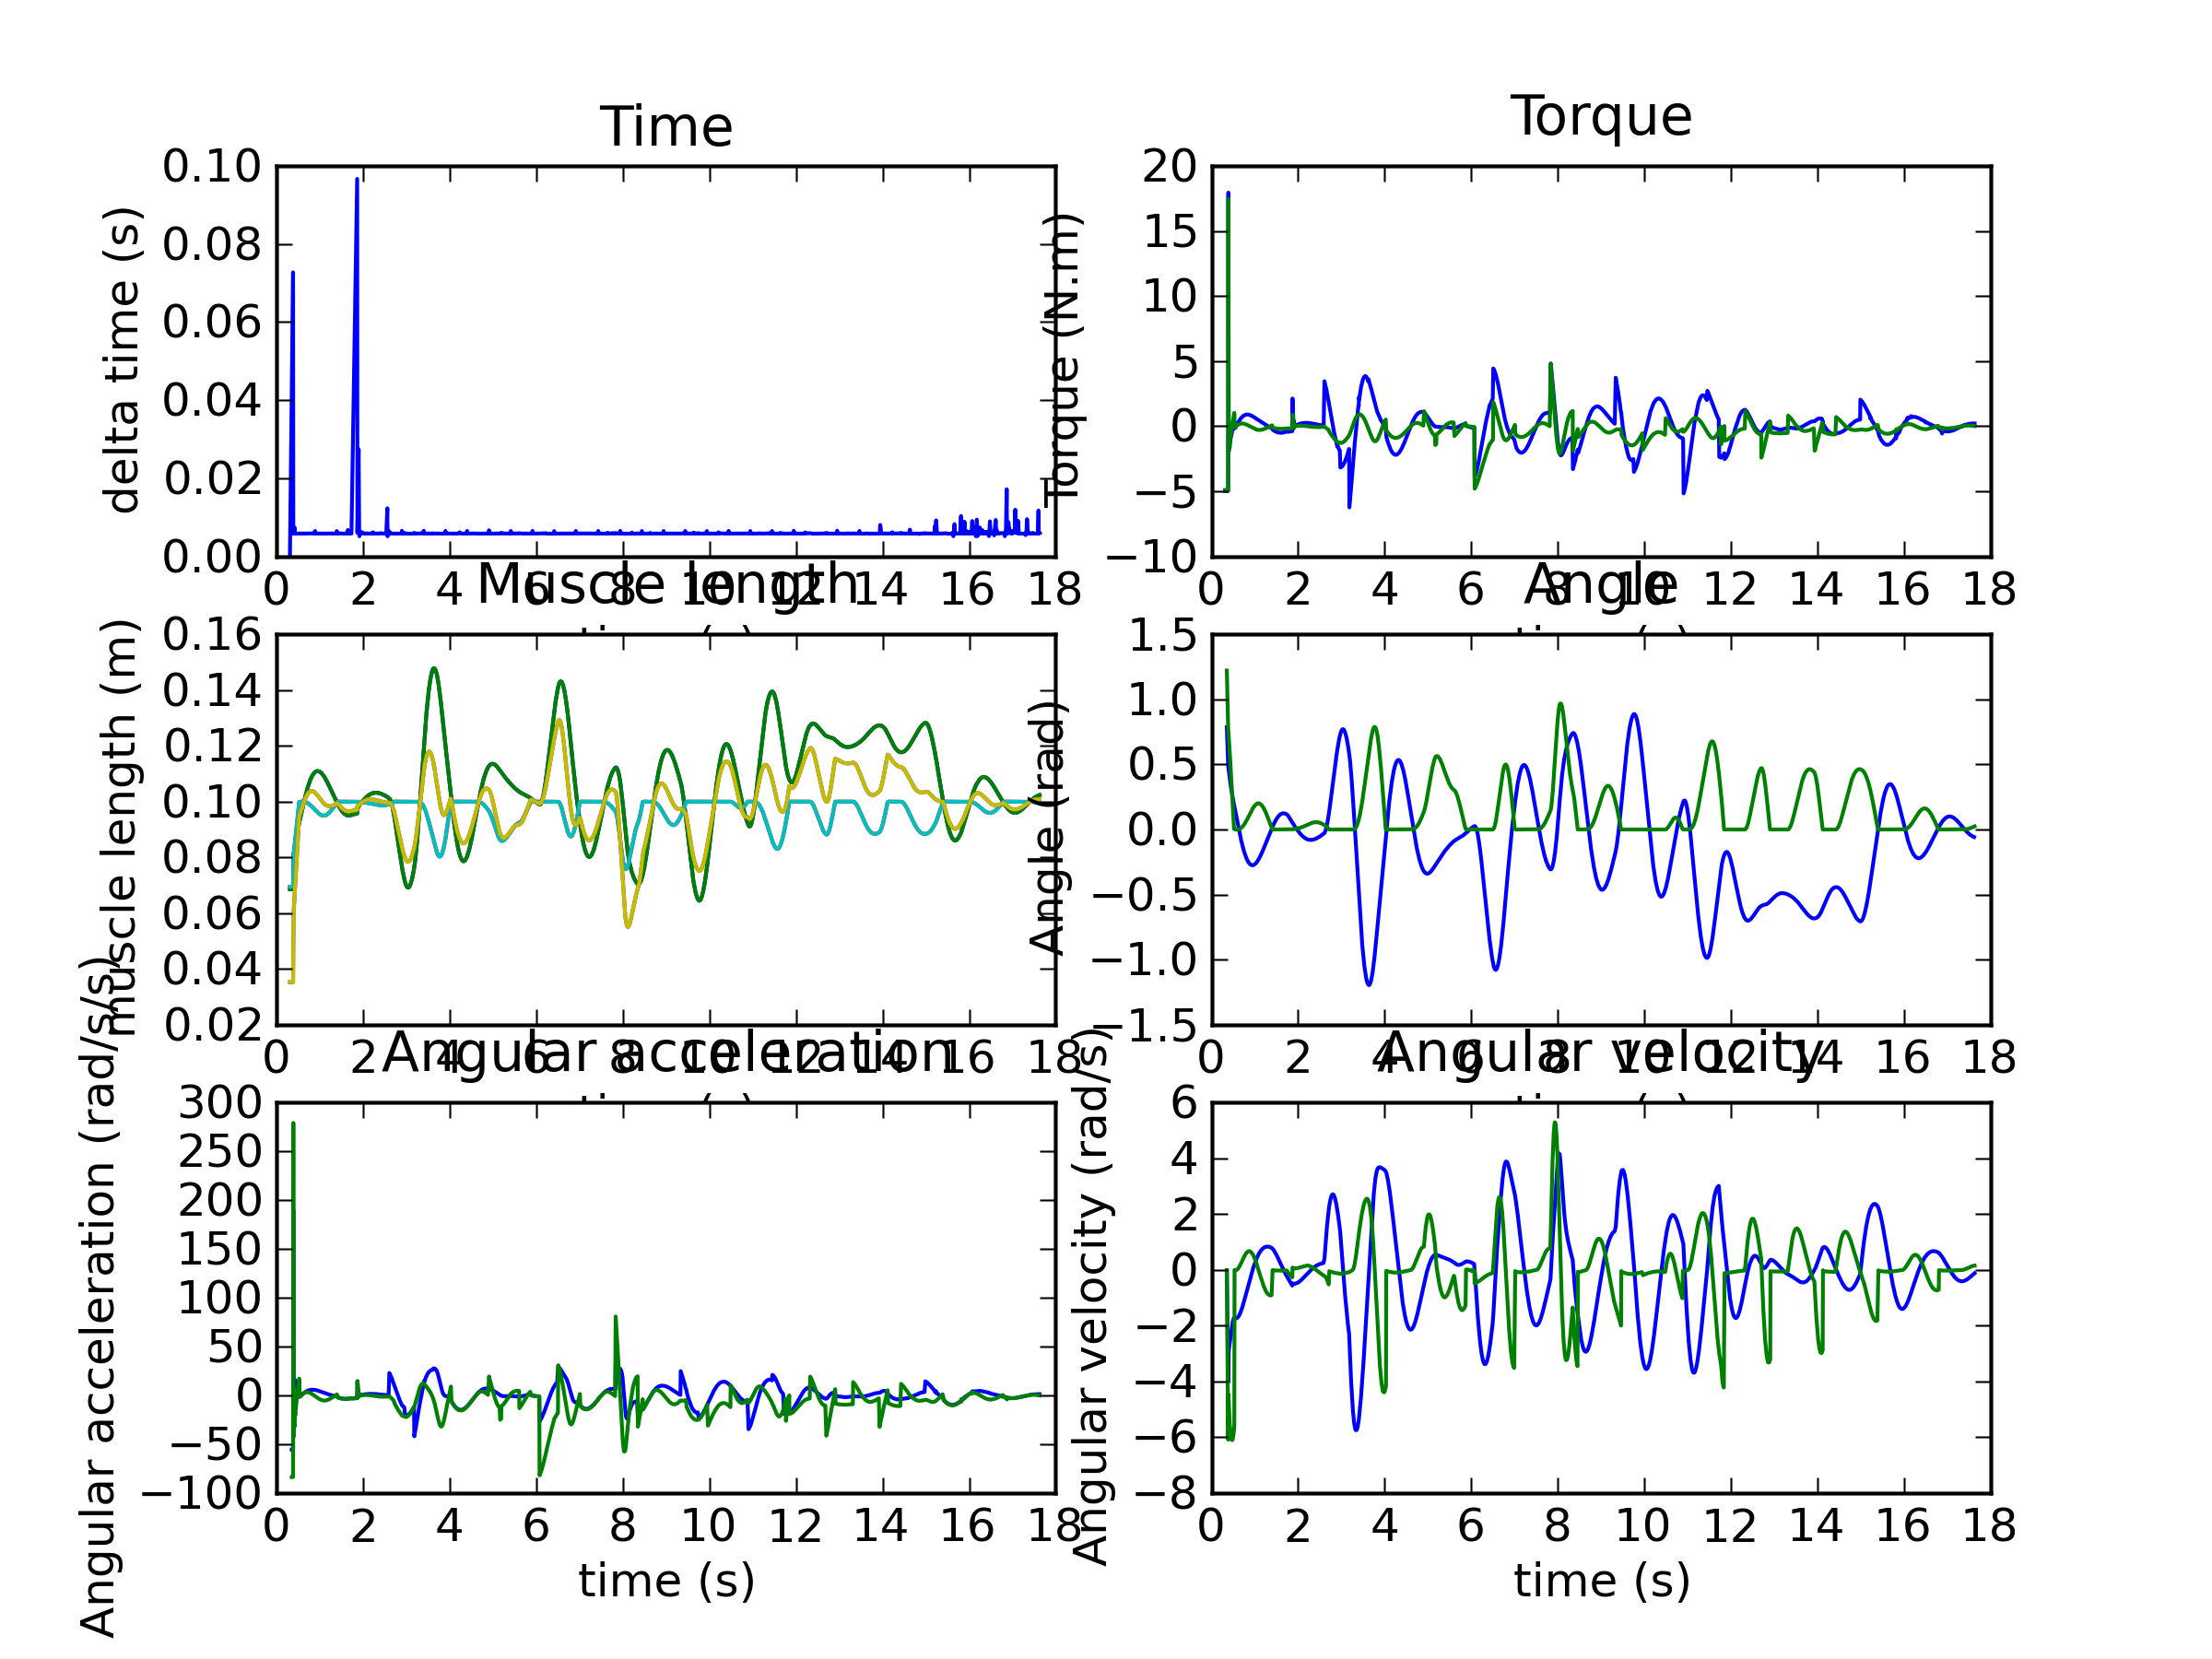
\includegraphics[width=.50\linewidth]{fig/pyarm2}}~~~
    \subfigure{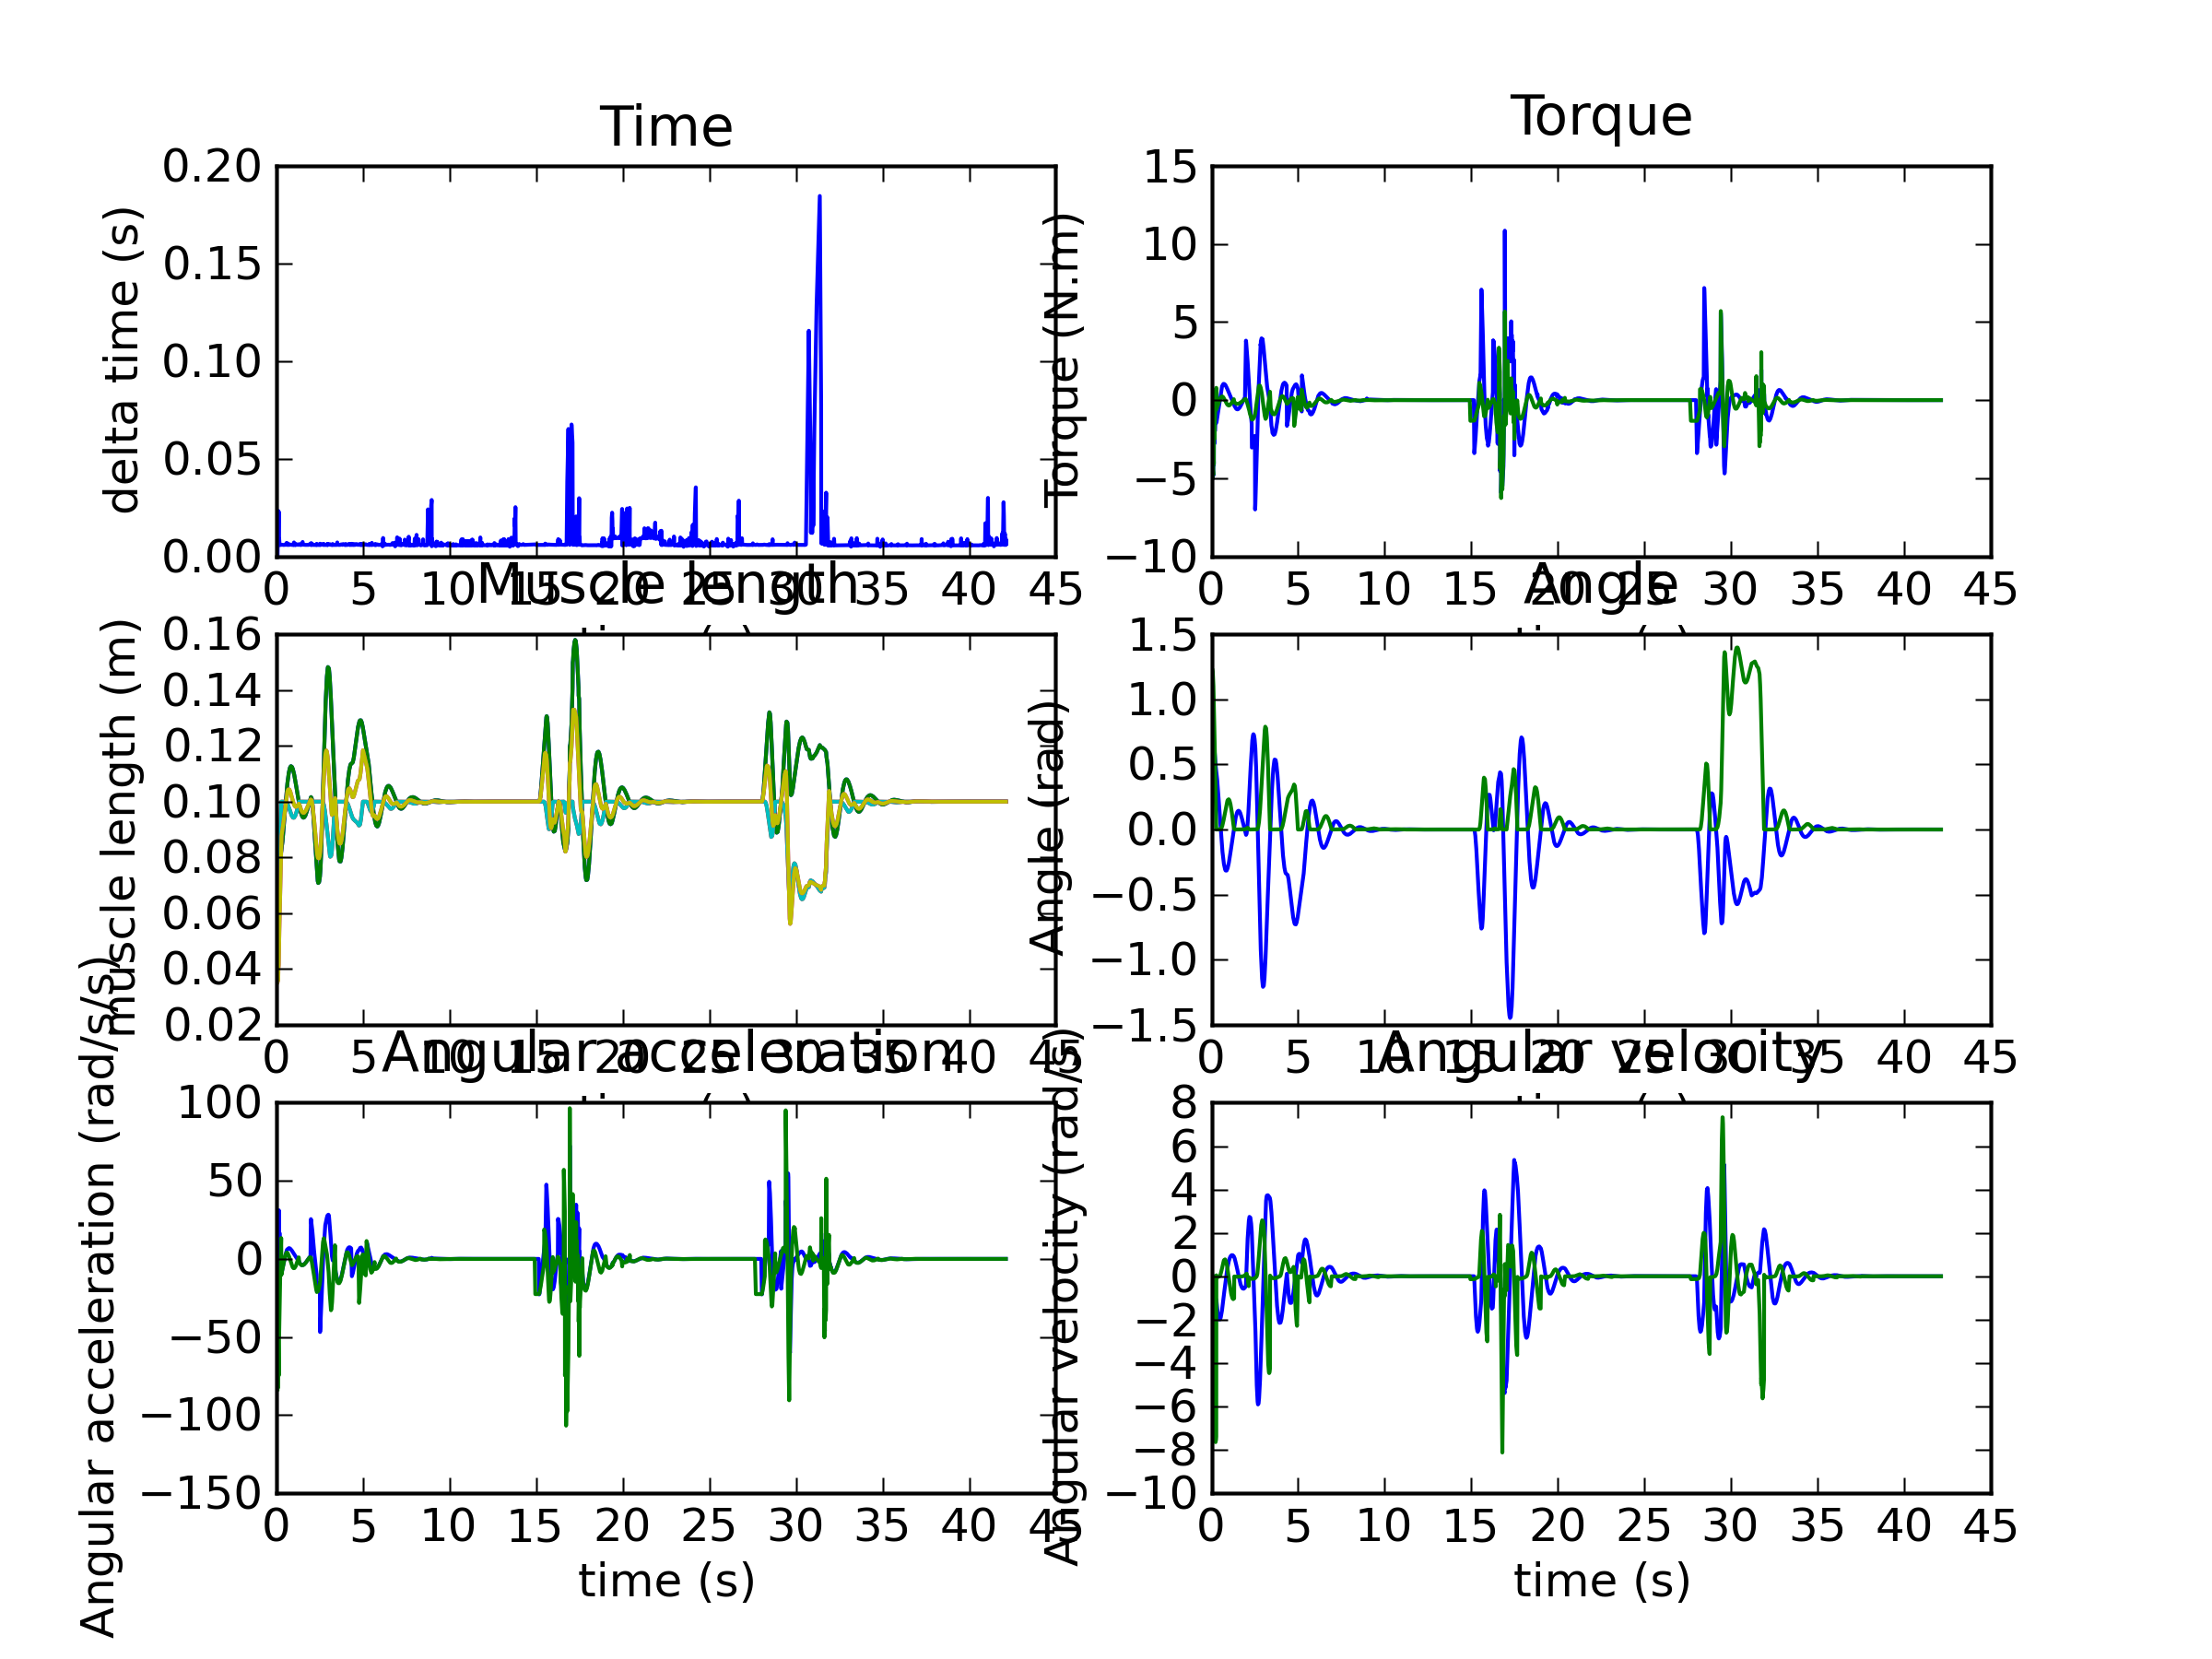
\includegraphics[width=.50\linewidth]{fig/pyarm3}}~~~
\end{figure}

\paragraph{}
Le simulateur est composé de 5 modules :
\begin{itemize}
    \item Filtre sur signal d'entrée
    \item Modèle de bras
    \begin{itemize}
        \item Cinématique
        \item Dynamique
    \end{itemize}
    \item Modèle de muscle
    \begin{itemize}
        \item Cinématique inverse
        \item Dynamique
    \end{itemize}
\end{itemize}

\paragraph{}
\begin{center}
        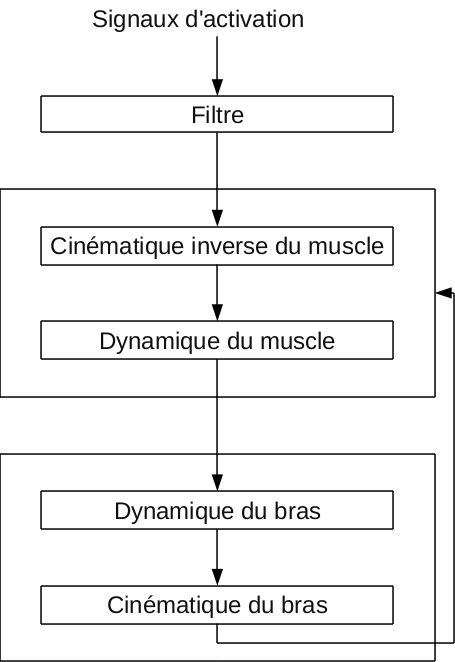
\includegraphics[width=.60\linewidth]{fig/modules}
\end{center}

%%%%%%%%%%%%%%%%%%%%%%%%%%%%%%%%%%%%%%%%%%%%%%%%%%%%%%%%%%%%%%%%%%%%%%%%%%%%%%%%

\section{Cinématique inverse du muscle}

\subsection{Résolution numérique par la méthode d'Euler}

Cette méthode de résolution numérique est la plus simple : elle se base sur la discrétisation de l'intervalle d'étude en un certain nombre de pas.

\[l = l_m - A q\]
\[\dot{l} = \frac{\delta l}{\delta t}\]

\begin{tabular}{lcl}
    $l_{m}$   & = & Longueur du muscle $i$ au repos pour l'angle $q = 0$ \\
\end{tabular}
    
\begin{center}
        \includegraphics[width=.50\linewidth]{fig/moment_arm}
\end{center}

% TODO
Dans les modèles de Mitrovic et Kambara, la longueur du bras d'inertie est constante. Elle correspond au rayon ...
Sous réserve que la longueur de l'arc soit toujours positive (...)
% TODO

\begin{center}
        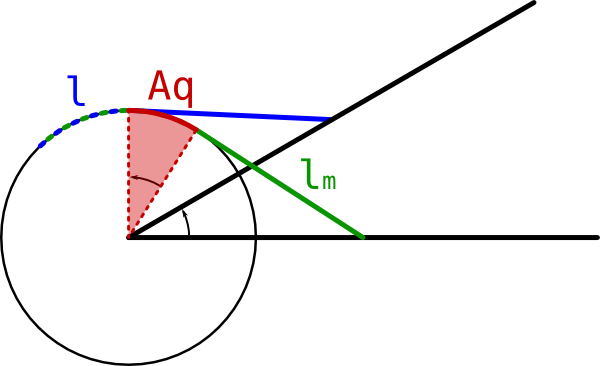
\includegraphics[width=.50\linewidth]{fig/muscle_length}
\end{center}

%%%%%%%%%%%%%%%%%%%%%%%%%%%%%%%%%%%%%%%%%%%%%%%%%%%%%%%%%%%%%%%%%%%%%%%%%%%%%%%%

\section{Dynamique du muscle}

\subsection{Katayama (Mitrovic et Kambara)}

\paragraph{}
Mitrovic~:
\[ \tau = -A^T t(l_m, \dot{l_m}, \tilde{u}) \]
\[ t(l_m, \dot{l_m}, \tilde{u}) = k(\tilde{u}) \cdot (l_r(\tilde{u}) - l_m) + b(\tilde{u}) \cdot \dot{l_m} \]

\paragraph{}
Kambara~:
\[ \tau = A^T t(l_m, \dot{l_m}, \tilde{u}) \]
\[ t(l_m, \dot{l_m}, \tilde{u}) = -k(\tilde{u}) \cdot (l_r(\tilde{u}) - l_m) + b(\tilde{u}) \cdot \dot{l_m} \]

\paragraph{}
\begin{tabular}{lcl}
    $k(\tilde{u})$    & = & $k_0 + k \cdot \tilde{u}$ \\
    $b(\tilde{u})$    & = & $b_0 + b \cdot \tilde{u}$ \\
    $l_r(\tilde{u})$  & = & $l_0 - r \cdot \tilde{u}$ \\
\end{tabular}

\begin{tabular}{lcl}
    $L_i^{rest}(\tilde{u}_i)$ & = & $l_{0i}^{rest} - l_{1i}^{rest} \tilde{u}_i$ \\
    %$L_i$ & = & $l_{0i} - \sum_{j=1}^2 A_{i,j} q_j $ \\
\end{tabular}

\paragraph{}
\begin{tabular}{lcl}
    $\tau_i \in \mathbb{R}^2$            & = & Couple total exercé sur les articulations \\
    $A \in \mathbb{R}^{6 \times 2}$      & = & Matrice des bras de levier \\
    $t(l, \dot{l}, u) \in \mathbb{R}^6$  & = & Tension exercée par les muscles \\
    \\

    $k(\tilde{u}) \in \mathbb{R}^6$      & = & Raideur des muscles \\ % élasticité
    $k_0 \in \mathbb{R}^6$               & = & Raideur intrinsèque des muscles $(N/m)$ \\
    $\mathrm{k} \in \mathbb{R}^6$                 & = & Coefficient de variation de l'élasticité des muscles $(N/m)$ \\
    \\

    $\nu(\tilde{u}) \in \mathbb{R}^6$    & = & Viscosité des muscles \\
    $\nu_0 \in \mathbb{R}^6$             & = & Viscosité intrinsèque des muscles $(N \cdot s/m)$ \\
    $\mathrm{\nu} \in \mathbb{R}^6$               & = & Coefficient de variation de la viscosité des muscles $(N \cdot s/m)$ \\
    \\

    $l_r(\tilde{u}) \in \mathbb{R}^6$    & = & Longueur des muscles au repos \\
    $l_{r0} \in \mathbb{R}^6$            & = & Longueur des muscles au repos \\
    $\mathrm{r} \in \mathbb{R}^6$                 & = & Coefficient de variation de la longueur des muscles au repos \\
    \\

    $l_m \in \mathbb{R}^6$               & = & Longueur des muscles \\
    $l^{rest}_{1i} \in \mathbb{R}^6$     & = & Coefficient de variation de la longueur des muscles au repos \\
    $l_{0} \in \mathbb{R}^6$                  & = & Longueur du muscle $i$ au repos pour l'angle $q = 0$ \\
    %$l_{0} \in \mathbb{R}^6$                 & = & Longueur du muscle au repos pour l'angle $q = 0$ \\
    \\

    $u \in \mathbb{R}^6$                 & = & Signaux d'activation des muscles \\
    $\tilde{u} \in \mathbb{R}^6$         & = & Signaux d'activation filtrés \\
\end{tabular}

\paragraph{}
Mitrovic \cite{katayama1993} (p.356-357)~: 
\[
A =
\begin{pmatrix}
    0.04 & 0.04 & 0     & 0     & 0.028 & 0.035 \\
    0    & 0    & 0.025 & 0.025 & 0.028 & 0.035 \\
\end{pmatrix}^T
\]

\begin{tabular*}{1.0\textwidth}{@{\extracolsep{\fill}}|l|r|r|r|r|r|r|}
%\begin{tabular}{|l|m{5em}|m{5em}|m{5em}|m{5em}|m{5em}|m{5em}|}
    \hline
                            & $k$    & $k_0$ & $\nu$ & $\nu_0$ & -       & - \\
    \hline
    fléchisseur de l'épaule & 1621.6 & 810.8 & 108.1 & 54.1    & -3.491  &  9.076 \\
    \hline
    extenseur de l'épaule   & 1621.6 & 810.8 & 108.1 & 54.1    &  3.491  & -2.793 \\
    \hline
    fléchisseur du coude    & 1621.6 & 810.8 & 108.1 & 54.1    & -2.182  &  5.672 \\
    \hline
    extenseur du coude      & 1621.6 & 810.8 & 108.1 & 54.1    &  2.182  &  0.436 \\
    \hline
    double fléchisseur      & 1621.6 & 810.8 & 108.1 & 54.1    & -5.498  &  14.294 \\
    \hline
    double extenseur        & 1621.6 & 810.8 & 108.1 & 54.1    &  5.498  & -1.343 \\
    \hline
\end{tabular*}

\paragraph{}
Kambara  \cite{kambara2009} (p.359-360)~:
\[
A =
\begin{pmatrix}
    0.04 & -0.04 & 0     & 0      & 0.028 & -0.035 \\
    0    & 0     & 0.025 & -0.025 & 0.028 & -0.035 \\
\end{pmatrix}^T
\]

\begin{tabular*}{1.0\textwidth}{@{\extracolsep{\fill}}|l|r|r|r|r|r|r|}
%\begin{tabular}{|l|m{5em}|m{5em}|m{5em}|m{5em}|m{5em}|m{5em}|}
    \hline
                            & $k$    & $k_0$  & $\nu$ & $\nu_0$ & -      & - \\
    \hline
    fléchisseur de l'épaule & 1000   & 3000   & 50    & 100     & 0.15   & 0.077 \\
    \hline
    extenseur de l'épaule   & 1000   & 2000   & 50    & 100     & 0.15   & 0.128 \\
    \hline
    fléchisseur du coude    & 600    & 1400   & 50    & 100     & 0.15   & 0.100 \\
    \hline
    extenseur du coude      & 600    & 1200   & 50    & 100     & 0.15   & 0.040 \\
    \hline
    double fléchisseur      & 300    & 600    & 50    & 100     & 0.15   & 0.020 \\
    \hline
    double extenseur        & 300    & 600    & 50    & 100     & 0.15   & 0.019 \\
    \hline
\end{tabular*}


%%%%%%%%

\subsection{Brown (Weiwei)}

\begin{center}
        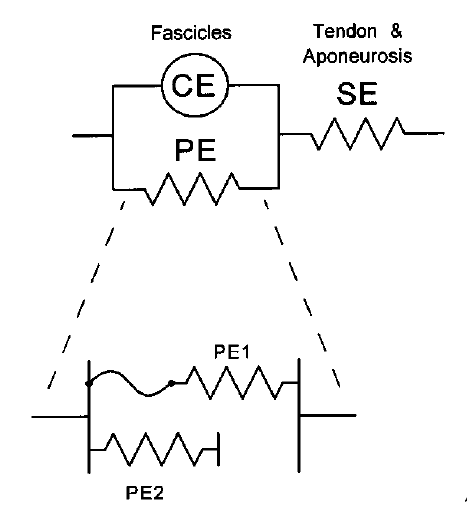
\includegraphics[width=.40\linewidth]{fig/brown}
\end{center}

\begin{tabular}{lcl}
    $CE$  & = & éléments contractiles \\
    $SE$  & = & élasticité des tendons (ignorée) \\
    $PE$  & = & élasticité du muscle \\
    $PE1$ & = & résistance à l'étirement du muscle passif \\
    $PE2$ & = & résistance à la compression du muscle actif \\
\end{tabular}

\paragraph{}
\begin{tabular}{lcl}
    $\tau$ & = & $M(q) T(a, l(q), v(q, \dot{q}))$ \\
    \\
    $T(a, l, v)$ & = & $A(a,l)(F_L(l) F_V(l,v) + F_P(l))$ \\
    $A(a, l)$    & = & $1 - \exp \left(- \left(\frac{a}{0.56 N_f(l)}\right)^{N_f(l)}\right)$ \\
    $N_f(l)$     & = & $2.11 + 4.16 \left(\frac{1}{l} - 1\right)$ \\
    $F_L(l)$     & = & $\exp \left(-\left|\frac{l^{1.93} - 1}{1.03}\right|^{1.87}\right)$ \\
    $F_V(l, v)$  & = & $\left\{ 
        \begin{array}{l}
            \frac{-5.72 - v}{-5.72 + (1.38 + 2.09 l) v}, v \leq 0 \\
            \frac{0.62 - \left(-3.12 + 4.21 l - 2.67 l^2\right) v}{0.62 + v}, v > 0 \\
        \end{array}
        \right.$ \\
    $F_P(l)$     & = & $-0.02 \exp(13.8 - 18.7 l)$ \\
\end{tabular}

\paragraph{}
\begin{tabular}{lcl}
    $M(q)$  & = & matrice des bras de levier $(a + b \cos (c q))$ \\
    $T(a, l, v)$ & = & tension exercée par le muscle \\
    $A(a, l)$    & = & relation activation-fréquence \\
%    $N_f(l)$     & = &  \\
    $F_L(l)$     & = & relation force-longueur \\
    $F_V(l, v)$  & = & relation force-vitesse \\
    $F_P(l)$     & = & force élastique du muscle \\ % TODO ???
    $a$          & = & signaux d'activation filtrés du muscle \\
    $l$          & = & longueur du muscle \\
    $v$          & = & vitesse de contraction du muscle \\
\end{tabular}


%%%%%%%%%%%%%%%%%%%%%%%%%%%%%%%%%%%%%%%%%%%%%%%%%%%%%%%%%%%%%%%%%%%%%%%%%%%%%%%%

\section{Modèle du bras}

%%%%%%%%

\subsection{Cas général}

Dynamique inverse~:
%\begin{equation}
%\label{dynamique inverse}
%\tau = M(q)\ddot{q} + C(q, \dot{q}) + B(\dot{q}) + G(q)
%\end{equation}
\[\tau = M(q)\ddot{q} + C(q, \dot{q}) + B(\dot{q}) + G(q)\]

Dynamique~:
\[\Leftrightarrow \ddot{q} = M(q)^{-1} (\tau - C(q, \dot{q}) - B(\dot{q}) - G(q))\]
%\[
%(\ref{dynamique inverse}) \Leftrightarrow \ddot{q} = M(q)^{-1} (\tau - C(q, \dot{q}) - B(\dot{q}) - G(q))
%\]

\begin{tabular}{lcl}
    $M(q) \in \mathbb{R}^{2 \times 2}$  & = & matrice des moments d'inertie \\ % TODO
    $C(q, \dot{q}) \in \mathbb{R}^{2}$  & = & force de Coriolis et force centripète \\
    $B(\dot{q}) \in \mathbb{R}^{2}$     & = & force de viscosité et de friction \\ % TODO
    $G(q) \in \mathbb{R}^{2}$           & = & force de gravité \\
    $\tau \in \mathbb{R}^{2}$           & = & couple total exercé sur les articulations ($N \cdot m$) \\
    $\ddot{q} \in \mathbb{R}^{2}$       & = & accélération angulaire ($rd \cdot s^{-2}$) \\
    $\dot{q} \in \mathbb{R}^{2}$        & = & vitesse angulaire ($rd \cdot s^{-1}$)\\
    $q \in \mathbb{R}^{2}$              & = & angle ($rd$)\\
\end{tabular}

\subsection{Modèles étudiés}

\begin{tabular}{|c|l|l|}
    \hline
    Mitrovic & $\tau = M(q)\ddot{q} + C(q, \dot{q})$
             & $\ddot{q} = M(q)^{-1} (\tau - C(q, \dot{q}))$ \\
    \hline
    Kambara  & $\tau = M(q)\ddot{q} + C(q, \dot{q}) + G(q)$
             & $\ddot{q} = M(q)^{-1} (\tau - C(q, \dot{q}) - G(q))$ \\
    \hline
    Weiwei   & $\tau = M(q)\ddot{q} + C(q, \dot{q}) + B(\dot{q})$
             & $\ddot{q} = M(q)^{-1} (\tau - C(q, \dot{q}) - B(\dot{q}))$ \\
    \hline
\end{tabular}

\paragraph{}
\begin{tabular}{lcl}
    $M(q)$ & = &
    $
    \begin{pmatrix}
        d_1 + 2 d_2 \cos(q_e)  & d_3 + d_2 \cos(q_e) \\
        d_3 + d_2 \cos(q_e) & d_3 \\
    \end{pmatrix}
    $ \\

    $C(q, \dot{q})$ & = &
    $
    \begin{pmatrix}
        -\dot{q}_e (2 \dot{q}_s + \dot{q}_e) \\
        \dot{q}_s^2 \\
    \end{pmatrix}
    d_2 \sin(q_e)
    $\\

    $B(\dot{q})$ & = &
    $
    \begin{pmatrix}
        0.05  & 0.025 \\
        0.025 & 0.05 \\
    \end{pmatrix}
    \dot{q}
    $\\

    $G(q)$ & = &
    $
    \begin{pmatrix}
        m_u \hat{g}  \gamma_u \cos(q_s) + m_f \hat{g} (l_u \cos(q_s) + \gamma_f \cos(q_s + q_e)) \\
        m_f \hat{g}  \gamma_f \cos(q_s + q_e) \\
    \end{pmatrix}
    $ \\

    \\
    $d_1$ & = & $\iota_s + \iota_e + m_f l_u^2$ \\
    $d_2$ & = & $m_f l_u \gamma_f$ \\
    $d_3$ & = & $\iota_e$ \\
    \\
    $m_i$ & = & masse du membre $i$ ($kg$) \\
    $l_i$ & = & longueur du membre $i$ ($m$) \\
    $\gamma_i$ & = & distance séparant le centre de l'articulation au centre de masse du membre $i$ ($m$) \\
    $\iota_j$ & = & moment d'inertie de l'articulation $j$ ($kg \cdot m^2$) \\
    $\hat{g}$ & = & champ de pesanteur ($m \cdot s^{-2}$) \\
    \\
%Indices :\\

    $u$ & = & bras (supérieur)\\
    $f$ & = & avant-bras\\

    $s$ & = & épaule\\
    $e$ & = & coude\\
\end{tabular}

\paragraph{}
\begin{small}
\begin{tabular}{|c|c|c|c|c|c|c|c|c|c|}
    \hline
             & $m_u$  & $m_f$  & $l_u$ & $l_f$  & $\gamma_u$ & $\gamma_f$ & $\iota_s$            & $\iota_f$            & $\hat{g}$ \\
    \hline
    Mitrovic \cite{katayama1993} (p.356) 
             & $1.59$ & $1.44$ & $0.3$ & $0.35$ & $0.18$     & $0.21$     & $4.77 \cdot 10^{-2}$ & $5.88 \cdot 10^{-2}$ & - \\
    \hline
    Kambara  \cite{kambara2009} (p.359)
             & $1.59$ & $1.44$ & $0.3$ & $0.35$ & $0.18$     & $0.21$     & $6.78 \cdot 10^{-2}$ & $7.99 \cdot 10^{-2}$ & N/A \\
    \hline
    Weiwei   \cite{li2006} (p.23)
             & $1.4$  & $1.1$  & $0.3$ & $0.33$ & $0.11$     & $0.16$     & $2.5 \cdot 10^{-2}$  & $4.5 \cdot 10^{-2}$  & - \\
    \hline
\end{tabular}
\end{small}

%%%%%%%%%%%%%%%%%%%%%%%%%%%%%%%%%%%%%%%%%%%%%%%%%%%%%%%%%%%%%%%%%%%%%%%%%%%%%%%%

\section{Cinématique du bras}

\subsection{Résolution numérique par la méthode d'Euler}

Cette méthode de résolution numérique est la plus simple : elle se base sur la discrétisation de l'intervalle d'étude en un certain nombre de pas.

\[\dot{q} = \delta \ddot{q} \cdot \delta t\]
\[q = \delta \dot{q} \cdot \delta t\]

%%%%%%%%%%%%%%%%%%%%%%%%%%%%%%%%%%%%%%%%%%%%%%%%%%%%%%%%%%%%%%%%%%%%%%%%%%%%%%%%

\section{Annexe}

\subsection{Modèle du bras}

%%%%%%%%

\subsubsection{Mitrovic}
Écriture originale \cite{katayama1993} (p.355).

\begin{align*}
    \begin{pmatrix}
        \tau_s \\
        \tau_e \\
    \end{pmatrix} =
    & \begin{pmatrix}
        \iota_s + \iota_e + m_f l_u^2 + 2 m_f l_u \gamma_f \cos(q_e)  &  \iota_e + m_f l_u \gamma_f \cos(q_e) \\
        \iota_e + m_f l_u \gamma_f \cos(q_e)  &  \iota_e\\
    \end{pmatrix}
    \begin{pmatrix}
        \ddot{q}_s \\
        \ddot{q}_e \\
    \end{pmatrix}\\
    & + m_f l_u \gamma_f \sin(q_e)
    \begin{pmatrix}
        -2 \dot{q}_e  &  -\dot{q}_e \\
        \dot{q}_s     &  0\\
    \end{pmatrix}
    \begin{pmatrix}
        \dot{q}_s \\
        \dot{q}_e \\
    \end{pmatrix}
\end{align*}

$
\Leftrightarrow 
\left \{
    \begin{tabular}{rcl}
        $\tau$ & = &
        $M(q)\ddot{q} + C(q, \dot{q})$ \\

        $M(q)$
        & = &
        $
        \begin{pmatrix}
            \iota_s + \iota_e + m_f l_u^2 + 2 m_f l_u \gamma_f \cos(q_e)  &  \iota_e + m_f l_u \gamma_f \cos(q_e) \\
            \iota_e + m_f l_u \gamma_f \cos(q_e)  &  \iota_e\\
        \end{pmatrix}
        $
        \\

        $C(q, \dot{q})$
        & = &
        $
        m_f l_u \gamma_f \sin(q_e)
        \begin{pmatrix}
            -2 \dot{q}_e  &  -\dot{q}_e \\
            \dot{q}_s     &  0\\
        \end{pmatrix}
        \begin{pmatrix}
            \dot{q}_s \\
            \dot{q}_e \\
        \end{pmatrix}
        $
        \\
    \end{tabular}
\right .
$

$
\Leftrightarrow 
\left \{
    \begin{tabular}{rcl}
        $\tau$ & = &
        $M(q)\ddot{q} + C(q, \dot{q})$ \\

        $M(q)$ & = &
        $
        \begin{pmatrix}
            d_1 + 2 d_2 \cos(q_e)  & d_3 + d_2 \cos(q_e) \\
            d_3 + d_2 \cos(q_e) & d_3 \\
        \end{pmatrix}
        $ \\

        $C(q, \dot{q})$ & = &
        $
        \begin{pmatrix}
            -\dot{q}_e (2 \dot{q}_s + \dot{q}_e) \\
            \dot{q}_s^2 \\
        \end{pmatrix}
        d_2 \sin(q_e)
        $\\

        $d_1$ & = & $\iota_s + \iota_e + m_f l_u^2$ \\
        $d_2$ & = & $m_f l_u \gamma_f$ \\
        $d_3$ & = & $\iota_e$ \\
    \end{tabular}
\right .
$

%%%%%%%%

\subsubsection{Kambara}
Écriture originale \cite{kambara2009} (p.360).

\begin{align*}
    \begin{pmatrix}
        \tau_s \\
        \tau_e \\
    \end{pmatrix}
    & = \begin{pmatrix}
        M_{11}\ddot{q}_s + M_{12}\ddot{q}_e + h_{122}\dot{q}_e^2 + 2h_{112}\dot{q}_s\dot{q}_e + g_1 \\
        M_{21}\ddot{q}_s + M_{22}\ddot{q}_e + h_{211}\dot{q}_s^2 + g_2 \\
    \end{pmatrix}\\
    & = \begin{pmatrix}
        M_{11}\ddot{q}_s + M_{12}\ddot{q}_e \\
        M_{21}\ddot{q}_s + M_{22}\ddot{q}_e \\
    \end{pmatrix} +
    \begin{pmatrix}
        h_{122}\dot{q}_e^2 + 2h_{112}\dot{q}_s\dot{q}_e \\
        h_{211}\dot{q}_s^2 \\
    \end{pmatrix} +
    \begin{pmatrix}
        g_1 \\
        g_2 \\
    \end{pmatrix}\\
    & = M(q) \ddot{q} + C(q, \dot{q}) + G(q)
\end{align*}

\paragraph{}
\begin{tabular}{lcl}
    $M(q)$ & = &
    $
    \begin{pmatrix}
        M_{11} & M_{12} \\
        M_{21} & M_{22} \\
    \end{pmatrix}
    $ \\

    $C(q, \dot{q})$ & = &
    $
    \begin{pmatrix}
        -d_2 \sin(q_e) \dot{q}_e^2 - 2 d_2 \sin(q_e)\dot{q}_s\dot{q}_e \\
        d_2 \sin(q_e) \dot{q}_s^2 \\
    \end{pmatrix} =
    \begin{pmatrix}
        -\dot{q}_e (2 \dot{q}_s + \dot{q}_e) \\
        \dot{q}_s^2 \\
    \end{pmatrix}
    d_2 \sin(q_e)
    $\\

    $G(q)$ & = &
    $
    \begin{pmatrix}
        g_1 \\
        g_2 \\
    \end{pmatrix}
    $ \\
    \\

    $M_{11}$ & = & $\iota_s + \iota_e + m_f(l_u^2 + 2 l_u \gamma_f \cos(q_e)) = d_1 + 2 d_2 \cos(q_e)$ \\
    $M_{12}$ & = & $\iota_e + m_f l_u \gamma_f \cos(q_e) = d_3 + d_2 \cos(q_e)$ \\
    $M_{21}$ & = & $\iota_e + m_f l_u \gamma_f \cos(q_e) = d_3 + d_2 \cos(q_e)$ \\
    $M_{22}$ & = & $\iota_e = d_3$ \\
    $h_{122}$ & = & $-m_f l_u \gamma_f \sin(q_e)$ \\
    $h_{112}$ & = & $-m_f l_u \gamma_f \sin(q_e)$ \\
    $h_{211}$ & = & $m_f l_u  \gamma_f \sin(q_e)$ \\
    $g_1$ & = & $m_u \hat{g}  \gamma_u \cos(q_s) + m_f \hat{g} (l_u \cos(q_s) + \gamma_f \cos(q_s + q_e))$ \\
    $g_2$ & = & $m_f \hat{g}  \gamma_f \cos(q_s + q_e)$ \\
    \\

    $d_1$ & = & $\iota_s + \iota_e + m_f l_u^2$ \\
    $d_2$ & = & $m_f l_u \gamma_f$ \\
    $d_3$ & = & $\iota_e$ \\
\end{tabular}

%%%%%%%%

\subsubsection{Weiwei}
Écriture originale \cite{li2006} (p.22).

\paragraph{}
\begin{tabular}{lcl}
    $\tau$ & = & $M(q)\ddot{q} + C(q, \dot{q}) + B(\dot{q})$ \\
    \\

    $M(q)$ & = &
    $
    \begin{pmatrix}
        d_1 + 2 d_2 \cos(q_e)  & d_3 + d_2 \cos(q_e) \\
        d_3 + d_2 \cos(q_e) & d_3 \\
    \end{pmatrix}
    $ \\

    $C(q, \dot{q})$ & = &
    $
    \begin{pmatrix}
        -\dot{q}_e (2 \dot{q}_s + \dot{q}_e) \\
        \dot{q}_s^2 \\
    \end{pmatrix}
    d_2 \sin(q_e)
    $\\

    $B(\dot{q})$ & = &
    $
    \begin{pmatrix}
        0.05  & 0.025 \\
        0.025 & 0.05 \\
    \end{pmatrix}
    \dot{q}
    $ \\
    \\

    $d_1$ & = & $\iota_s + \iota_e + m_f l_u^2$ \\
    $d_2$ & = & $m_f l_u \gamma_f$ \\
    $d_3$ & = & $\iota_e$ \\
\end{tabular}

%%%%%%%%%%%%%%%%%%%%%%%%%%%%%%%%%%%%%%%%%%%%%%%%%%%%%%%%%%%%%%%%%%%%%%%%%%%%%%%%

\section{Bibliographie}

%\cite{clef_de_référence}

\bibliographystyle{plain}
\bibliography{article}

\end{document}
